
\section{Formal definition of \lsystem}

\lsystem $L$ is formally triplet $L = (\Sigma, \omega, R)$, where

\begin{itemize*}
	\item $\Sigma$ is \emph{alphabet}, non-empty set of symbols, $\Sigma^{*}$ is set of all words\footnote{Word is a sequence of symbols.} which can be created from the alphabet $\Sigma$, $\Sigma^{+}$ is set of all non-empty words which can be created from the the alphabet $\Sigma$,
	\item $\omega \in \Sigma^{+}$ is \emph{axiom} (also called seed), word defining the initial state of the \lsystem,
	\item $R \subset \Sigma \times \Sigma^{*}$ is finite set of \emph{rewrite rules} (production rules), rewrite rule defining rewriting symbol $s \in \Sigma$ to word $w \in \Sigma^{*}$ is written as $s \rightarrow w$.
\end{itemize*}

For any symbol $s \in \Sigma$ which does not appear on the left hand side of any rewrite rule in $R$, the identity rewrite rule $s \rightarrow s$ is assumed.
These symbols are called constants or terminals.

Formal definition of \lsystem is similar to deterministic context-free grammar but there are few differences.
In grammar we distinguishes terminal and non-terminal symbols, but in \lsystems we do not define them explicitly (we define identity rewrite rule for terminal symbols in \lsystems).
Next difference is in initial string.
In grammar we have only one symbol as initial state but \lsystem allows non-empty word.
The biggest difference is in rewriting principles which is described is following section.


\subsection{Rewriting principles of \lsystem}

Starting with axiom (0th iteration) in each iteration \emph{all} symbols are rewritten with rewrite rules forming next iteration.
All symbols can be rewritten because every symbol is on the left side of some rewrite rule.
% (if symbol have not been on the left side of some rewrite rule, identity rule would be defined).
There is only one way how to rewrite symbols in iteration thus rewriting is deterministic, result depends only on axiom.

Rewriting of symbols is parallel (all symbols are rewritten at once).
This means that if some symbol is rewritten, resulting symbols are not rewritten again in the same iteration.

Described rewriting principles distinguishes \lsystem and formal grammar.
In grammar there is not mandatory to rewrite all possible symbols (derivation of start state can result in more different derivations).
Thus, \lsystems are strict subsets of languages.

\lsystem in \autoref{lsys:rrExample} produces strings shown in \autoref{fig:rrExampleResult}.
\lsystem starts with axiom $A$ and two rewrite rules $A \rightarrow B$ and $B \rightarrow A, B$.
In the first iteration axiom $A$ is rewritten by first rewrite rule to $B$.
In the second iteration is $B$ rewritten with second rewrite rule to symbols $A, B$.
In the third iteration is first symbol $A$ rewritten to $B$ and second symbol $B$ rewritten to $A, B$ which gives string $B, A, B$ and so on.

\begin{Lsystem}[label=lsys:rrExample,caption={Simple \lsystem as example of rewriting principles}]
lsystem RewritingExample {
	set symbols axiom = A;
	set iterations = 6;
	set interpretEveryIteration = true;
	@rewrite A to B;@
	@rewrite B to A B;@
}
process all with SymbolPrinter;
\end{Lsystem}

\begin{table}[h]
	\centering
	\begin{tabular}{c l}
   		\toprule
   		Iteration & String of symbols \\
   		\midrule
		0 & A \\
		1 & B \\
		2 & A B \\
		3 & B A B \\
		4 & A B B A B \\
		5 & B A B A B B A B \\
		6 & A B B A B B A B A B B A B \\
		\bottomrule
	\end{tabular}
	\caption{Result of \lsystem in \autoref{lsys:rrExample}}
	\label{fig:rrExampleResult}
\end{table}


\subsection{Interpretation of \lsystem symbols}

Result of \lsystem rewriting is string of symbols.
As it was mentioned in the \nameref{sec:Introduction} we can interpret string of symbols in any way for example as computer graphics or music.

The most common and the simplest interpretation of \lsystem symbols is interpret them as 2D graphics elements like lines or polygons.
This interpretation is often called \emph{turtle graphics} and it will be used in the most \lsystems in this thesis.
This approach can be easily extended into 3D.

Let symbol \texttt{F} is interpreted as \emph{draw line forward}, \texttt{+} as \emph{turn left} and \texttt{-} as turn right.
\autoref{fig:intSequences} shows interpreted strings of symbols.
Initial direction is to the right.

\begin{figure}[h]
	\centering
	\subfloat[\texttt{F + F - - F + F}, turning angle: $60^{\circ}$]{
		
\includegraphics[scale=1]{IntTriangle}
	} ~
	\subfloat[\texttt{F + F - F - F + F}, turning angle: $90^{\circ}$]{
		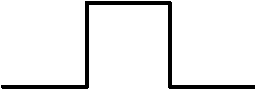
\includegraphics[scale=1]{IntSquare}
	} ~
	\subfloat[\texttt{F + F + + F - F - - F F - F}, turning angle: $60^{\circ}$]{
		\hspace{9mm}
\includegraphics[scale=1]{IntHexa}\hspace{9mm}
	}
	\caption{Examples of interpretation simple string of symbols}
	\label{fig:intSequences}
\end{figure}


More complex string of symbols as an example of interpretation is generated by \lsystem in \autoref{lsys:intExampleCode} where symbol $F$ is interpreted as \emph{draw line forward},
	symbol $+$ is interpreted as \emph{turn left} by 85 degrees and symbol $-$ as \emph{turn right} by 85 degrees (equally as \emph{turn left} by $-85$ degrees).
Result of interpretation of the first, second and fourth iteration is in \autoref{fig:intExample}.

\begin{Lsystem}[label=lsys:intExampleCode,caption={Symbol interpretation example}]
lsystem InterpretationExample {
	set symbols axiom = F;
	set iterations = 4;
	@interpret F as DrawForward(10);@
	@interpret + as TurnLeft(85);@
	@interpret - as TurnLeft(-85);@
	rewrite F to F + F - - F + F;
}
process all with SvgRenderer;
\end{Lsystem}

\begin{figure}[h]
	\subfloat{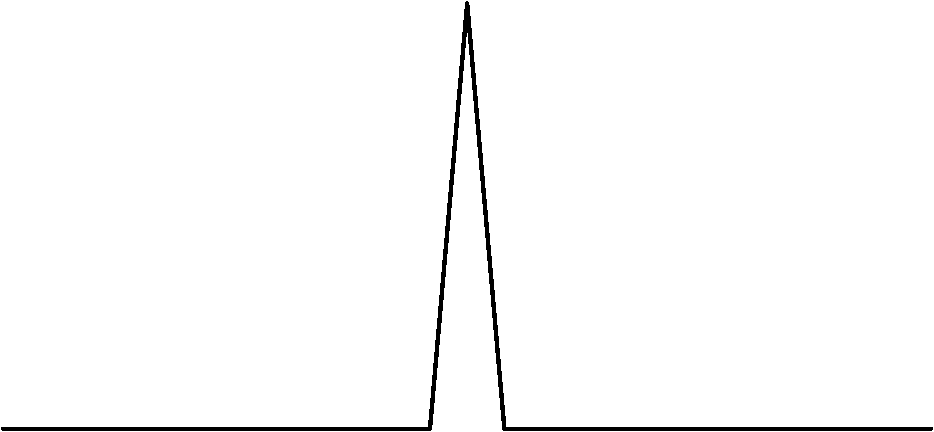
\includegraphics[scale=0.5]{Interpretation1}} \hfill
	\subfloat{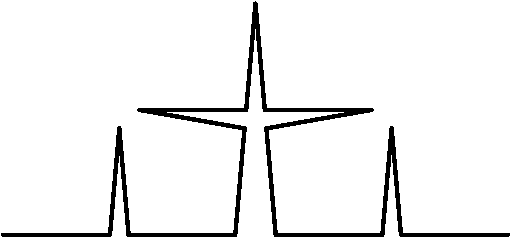
\includegraphics[scale=0.5]{Interpretation2}} \hfill
	\subfloat{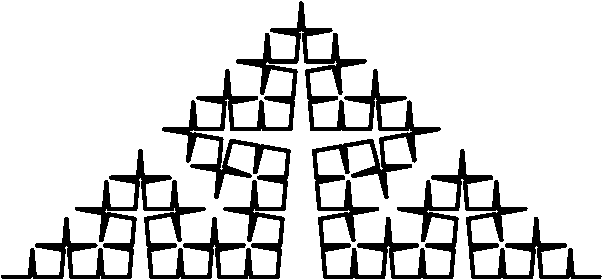
\includegraphics[scale=0.5]{Interpretation4}}
	\caption{The first, second and fourth iteration of the Cesaro curve (\autoref{lsys:intExampleCode})}
	\label{fig:intExample}
\end{figure}

\begin{figure}[h]
	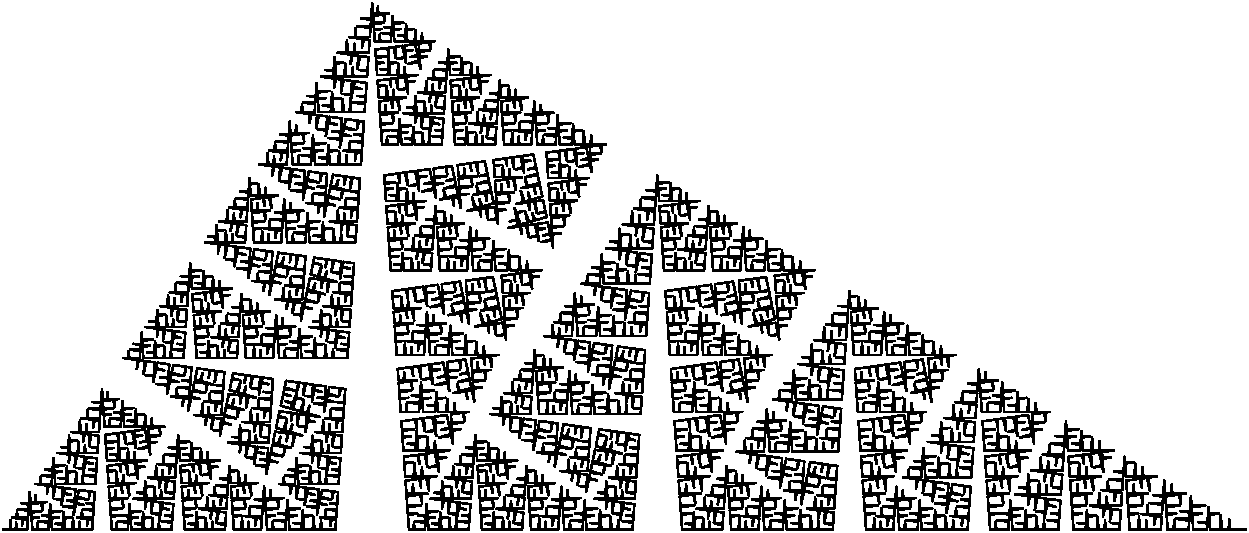
\includegraphics[width=1\linewidth]{RowOfTrees}
	\caption{Enhanced Cesaro curve from \autoref{fig:intExample} \cite[p.~48]{PL91}}
	\label{fig:rowOfTrees}
\end{figure}


































